%%% Example for master's thesis (in English)
\documentclass[english, dvipdfmx]{ampmt}             % pdflatex
%% \documentclass[dvipdfmx,english]{ampmt} % dvipdfmx

%%% Class options:
%%% chapter:   \chapter command is available (use report.cls).
%%% Options for article or report are also accepted.

%%% Title %%%%%%%%%%%%%%%%%%%%%%%%%%%%%%%%%%%%%%%%%%%%%%%%%%%%%%%%%%%%%%%%%%%%%%%
\title[Deep Reinforcement Learning for Optimal Self-Triggered Control]
      {Deep Reinforcement Learning for Optimal Self-Triggered Control}
      % [title for spine (option)]{title}
%%% Supervisors %%%%%%%%%%%%%%%%%%%%%%%%%%%%%%%%%%%%%%%%%%%%%%%%%%%%%%%%%%%%%%%%%
\supervisors{Yoshito OHTA}{Professor}             % First supervisor  {name}{title}
            {Kenji KASHIMA}{Assistant Professor} % Second supervisor {name}{title}
            {}{}                               % Third supervisor  {name}{title}
%%% Author %%%%%%%%%%%%%%%%%%%%%%%%%%%%%%%%%%%%%%%%%%%%%%%%%%%%%%%%%%%%%%%%%%%%%%
\author{Ibuki TAKEUCHI}
%%% Submission date %%%%%%%%%%%%%%%%%%%%%%%%%%%%%%%%%%%%%%%%%%%%%%%%%%%%%%%%%%%%%
\submissiondate{2021}{February}   % {year}{month}
%%% Width of a spine %%%%%%%%%%%%%%%%%%%%%%%%%%%%%%%%%%%%%%%%%%%%%%%%%%%%%
\setlength{\wdspine}{15mm}
%%% Number of output spines %%%%%%%%%%%%%%%%%%%%%%%%%%%%%%%%%%%%%%%%%%%%%%%%%%%%%
\def\numberofspines{1}
%%% Abstract %%%%%%%%%%%%%%%%%%%%%%%%%%%%%%%%%%%%%%%%%%%%%%%%%%%%%%%%%%%%%%%%%%%%
\abstract{%
  In this thesis, we construct the mathematical models of students who write
  the master's thesis and develop efficient algorithms for writing the master's
  thesis based on the models.
  We show that the proposed algorithms generate the thesis 65536 times
  more efficiently than writing by oneself.
}
%%% Packages and definitions of your own macros %%%%%%%%%%%%%%%%%%%%%%%%%%%%%%%%%
\newcommand{\rme}{\mathrm{e}}
%\usepackage[top=20truemm,bottom=20truemm,left=25truemm,right=25truemm]{geometry}
\usepackage{amsmath,ascmac,url,amsfonts,bm,here,algorithmic,algorithm,amsthm,color}
\newcommand{\argmax}{\mathop{\rm argmax}\limits}
\newcommand{\argmin}{\mathop{\rm argmin}\limits} 
\newcommand{\expect}{\mathbb{E}} 
\newcommand{\trans}[1]{#1^{\top}}
\newcommand{\pdif}[2]{\frac{\partial#1}{\partial#2}}
\newcommand{\odif}[2]{\frac{\rm{d}#1}{\rm{d}#2}}
\newtheorem{th.}{Th.}


%%% Control of output %%%%%%%%%%%%%%%%%%%%%%%%%%%%%%%%%%%%%%%%%%%%%%%%%%%%%%%%%%%

%%% If you don't want to output body text, activate the next line.
%% \outputbodyfalse

%%% If you don't want to output covers at the end of PDF, activate the next line.
%% \outputcoverfalse

%%% If you don't want to output abstract for submission at the end of PDF,
%%% activate the next line.
%% \outputabstractforsubmissionfalse

%%% If you want to change the layout, use \geometry command provided by
%%% the geometry package.
%% \geometry{hmargin=3cm,vmargin=2cm}

\begin{document}
\ifoutputbody
%%% Inside cover, abstract and table of contents %%%%%%%%%%%%%%%%%%%%%%%%%%%%%%%%
\makeinsidecover                % Inside cover
\makeabstract                   % Abstract
\maketoc                        % Table of contents
\setcounter{page}{1}
%%% Body %%%%%%%%%%%%%%%%%%%%%%%%%%%%%%%%%%%%%%%%%%%%%%%%%%%%%%%%%%%%%%%%%%%%%%%%
\section{Introduction}



\section{Preliminaries}
\subsection{Background of Deep Reinforcement Learning}
Consider a malkov decision process $M$ given with tuple $M=\{S,A,T,d_0,r,\gamma\}$. Here, $S,A$ denotes state, action set, and $T(s^{'}|s,a)$ express transition probability. Also, $d_0,r(s,a),\gamma\in[0,1]$ are distribution of initial state, reward, discount factor respectively. \par
Now, the purpose of reinforcement learning is to find a policy such that
\begin{equation}
	\pi^{*}=\argmax_{\pi}J(\pi) \label{purpose_of_rl}
\end{equation} 
where evaluation function $J(\pi)$ and (state) value function $V^{\pi}(s)$ is given as following:
\begin{align}
	V^{\pi}(s) &= \sum_{t=0}^{\infty}\gamma^tr(s_t, a_t)|_{a_t=\pi(s_t)}, s_0 = s\\
	J(\pi) &= \expect_{s_0\sim d_0}[V^{\pi}(s_0)]
\end{align}
Here, we define $Q$ function, which is useful tool for analyzing reinforcement learning. $Q$ function is given as 
\begin{align}
	Q^{\pi}(s,a) &= r(s, a) + \gamma\sum_{t=1}^{\infty}\gamma^tr(s_t, a_t)|_{a_t=\pi(s_t)} \nonumber\\
			    &= r(s, a) + \gamma V^{\pi}(s^{\prime}). \label{Q_func}
\end{align}
As showed in \eqref{Q_func}, $Q$ function express the value when agent select action $a$ freely and choose action according to the policy $\pi$ from next step. Thus, the $Q$-function is also known as the action value function.


\subsection{Policy Iteration}
There is an algorithm for achieving \eqref{purpose_of_rl}, called the policy iteration method. It consists in repeating the following two steps.
\begin{enumerate}
	\item Policy Evaluation: Find (or approximate) action value function $Q^{\pi}(s,a)$.
	\item Policy Improvement: Update policy as $\pi(s)=\argmax_aQ^{\pi}(s,a)$.
\end{enumerate}
It is known that the optimal policy $\pi^{*}$ can be obtained by repeating the above two steps (Policy Improvement Theorem).





\subsection{Algorithms adapted to the settings of state and action space}
\label{sec:policy_improvement}
In the case that both the state space and the action space take discrete values, it is easy to obtain
$\pi(s)=\argmax_aQ^{\pi}(s,a)$, which appeared in the previous section, by storing $Q^{\pi}(s,a)$ in a table.\par
Now, what about the case where the state space is continuous? Since the state $s$ takes a continuous value, it cannot be stored in a table. Therefore, Minh et al.\cite{DQN} took the approach of approximating $Q^{\pi}(s,a)$ by parametrizing it using a neural network. Since the action space is discrete, it is still possible to obtain $\argmax_aQ^{\pi}(s,a)$. \par
Finally, in the case whrere both state and action space is continuous, the problem is that it is very expensive to obtain $\argmax_aQ^{\pi}(s,a)$. Thus, up to this point, the policy $\pi$ has been determined by the Q-function, but this approach cannot be taken when both spaces are continuous. 
Therefore, the policy function is often parameterized as $\pi_{\theta}$ and the parameter $\theta$ is updated by gradient ascent. 

\subsection{Deterministic Policy Gradient Method}
Silver et al.\cite{DPG} finds the gradient for the evaluation function $J(\pi_{\theta})$, even if the policy $\pi(s)$ is defined as deterministic policy. This gradient is known as deteministic policy gradient(DPG), and it is calculate as following:
\begin{align}
	\nabla_{\theta}J(\pi_{\theta}) &= \expect_{s\sim\rho^{\pi_{\theta}}}[
	\nabla_{\theta}\pi_{\theta}(s)\nabla_{a}Q^{\pi_{\theta}}(s, a)|_{a=\pi_{\theta}(s)}] \label{true_pg} 
\end{align}
where, 
\begin{equation}
	\rho^{\pi_{\theta}}(s) = \int_{S}\sum_{t=0}^{\infty}\gamma^td_0(s_0)\textrm{Pr}(s_0\to s, t,  \pi_{\theta})\textrm{d}s_0
\end{equation}
is discounted distribution.\par
DDPG(Deep DPG) is a deep reinforcement learning algorithm which utilize this policy gradient. It adopts an Actor-Critic structure, and learns a critic network $Q(s,a|\omega)$ which approximates $Q^{\pi_{\theta}}$, and an actor network $\pi(s|\theta)=\pi_{\theta}$ which represents a measure $\pi$, respectively. The update algorithm of actor and critic is described below.\par
DDPG uses mini-batch learning. First, update idea of critic is shown. The purpose of critic is to approximate $Q^{\pi}$. Because $Q$ function is able to be decomposed like \eqref{Q_func}, $Q(s,a|\omega)$ should also be updated to satisfy this relation. For that, parameter $\omega$ is updated to the direction where it minimize Temporal Difference(TD) error: 
\begin{equation}
	\textrm{TD} = Q(s,a|\omega) - \{r(s,a)+\gamma Q(s,\pi(s)|\omega)\}
\end{equation}
Since it is difficult to optimize for whole $(s,a)$ at once, DDPG uses the mean squared error for the mini-batch $E$ as the loss function and reduces it. \par
Now, the above method of updating critic is supervised learning itself. Therefore, the data in the mini-batch must be i.i.d.. If the mini-batch $E$ uses the data of the last $N$ steps experienced by the agent, they are no longer independent. Hence, the agent stores the empirical data in a storage, called replay buffer, and randomly selects $N$ data from it to make a mini-batch to increase the variance of the mini-batch.\par
Next update law of actor are shown. Because actor is the representation of policy function $\pi(s)$, policy gradient is used for its update. However, since correct $Q$-function as in equation \eqref{true_pg} cannot be used in DDPG, approximated policy gradient
\begin{equation}
	\expect_{s\sim\rho^{\pi}}[\nabla_{\theta}\pi_{\theta}(s)\nabla_{a}Q(s, a|\omega)|_{a=\pi_{\theta}(s)}] \simeq \nabla_{\theta}J(\pi_{\theta}) 
\end{equation}
 is used. Furthurmore, an approximation to the expectation is made like following:
 \begin{equation}
	\expect_{s\sim\rho^{\pi}}[\nabla_{\theta}\pi_{\theta}(s)\nabla_{a}Q(s, a|\omega)|_{a=\pi_{\theta}(s)}] \simeq \frac{1}{N}\sum_{s\in E}[\nabla_{\theta}\pi_{\theta}(s)\nabla_{a}Q(s, a|\omega)|_{a=\pi_{\theta}(s)}]. \label{expectation_approximation}
\end{equation}
Therefore, the accuracy of the approximation of the policy gradient may be greatly degraded by the accuracy of critic approximation and the distribution of mini-batch.

\subsection{Exploration in DDPG}
\label{sec:exploration}
% 探索の必要性
% 探索ノイズの大小がDDPGにどのような影響を与えるのか
Reinforcement learning uses empirical data collected by interaction with the environment to improve a policy. An agent needs to take a variety of actions in each state in order to know better actions. This is called "exploration". When the action space is discrete, a exploration method called "$\varepsilon - greedy$" is widely known. \par
In the case of continuous action space, it is common to collect data with the action determined by adding noise $e$ to the output of the policy function during training, such as
\begin{equation}
	a = \pi_{\theta}(s) + e.
\end{equation}
(The noise-added policy is called the behavior policy in order to distinguish it from the learning policy.)Intuitively, the larger this noise is, the wider the exploration is expected to be. By increasing the distribution of behavioral data around $a=\pi_{\theta}(s)$, we can expect to improve the accuracy of approximating the gradient of the $Q$-function with respect to $a$. \par
Then, is it useful to enlarge the exploration noise in all cases? In DDPG, we stored the past empirical data in the replay buffer, and calculated the policy gradient using the data set selected with equal probability from them. Since the expected value of the policy gradient is taken for $s\sim\rho^{\pi_{\theta}}$, the state distribution of the replay buffer should be as close as possible to $\rho^{\pi_{\theta}}$. Adding a large exploration noise may violate this property in some cases. Therefore, it may be disadvantageous to increase the exploration noise. This is considered to be a kind of problem called the "exploration and exploitation dilemma".


\section{Problem Formulation}
\subsection{Self-Triggered Control}
We consider control system like Fig. \ref{image}.
\begin{figure}[h]
	\centering
 	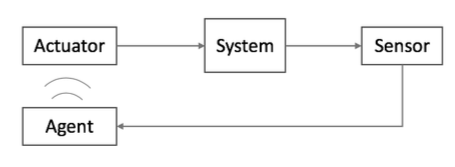
\includegraphics[width=10cm]{event.png}
 	\caption{control system} \label{image}
\end{figure}
Here, the control target is a continuous-time system as in Equation \eqref{continuous_system}
\begin{equation}
	\dot{s} = h(s,u) \label{continuous_system}
\end{equation}\par
Now, we consider a feedback control for system \eqref{continuous_system}. In this paper, we call the observation of the state variable $s$ and the sending of the input signal to the actuator as "interaction". In the self-triggered control, the agent does not make interaction continuously, but after a communication interval $\tau$ seconds determined by the agent itself. In order to express it mathematically, we assume that the agent's control law $\pi(s)$ is a vector-valued function consisting of two elements, where the first element represents the input $u$ sent to the actuator and the second element represents the interval $\tau (sec)$. The input $u$ sent in the previous interaction is added until the time of the next interaction (ZOH control).

\subsection{Optimal Self-Triggered Control}
The optimal self-triggered control law $\pi^{*}$ is defined as follows
\begin{align}
	\pi^{*} &= \argmax_{\pi}J(\pi) \label{optimal_policy}\\
	J(\pi) &= \expect_{s_0\in d_0}[V^{\pi}(s_0)] \\
	% V^{\pi}(s_0) &= \sum_{i=0}^{\infty} \gamma^i\{-s_i^{\top}Qs_i-\pi_1(s_i)^{\top}R\pi_1(s_i)+\lambda \pi_2(s_i)\} \\
	V^{\pi}(s_0) &= \sum_{i=0}^{\infty} \gamma^i r^{\pi}_i \label{value} \\
	r^{\pi}_i &= -\int_{T_i}^{T_{i+1}}s(t)^{\top}Qs(t)\textrm{d}t +\tau_ia_i^{\top}Ra_i + \lambda \tau_i, ~T_i = \sum_{l=0}^{i} \tau_l \label{reward}
\end{align}
where $i$ denote the number of interactions, and $a_i$ and $\tau_i$ be the outputs of the measures $\pi$ for the $i$th interaction, respectively. \par

\section{Reinforcement Learning for Optimal Self-Triggered Control}
In reinforcement learning, the agent is expected to perform interactions step by step. The self-triggered control problem considered in this paper, where the control target is given as a continuous-time system, satisfies the assumption of reinforcement learning by considering the communication with the actuator as one step.\par

\subsection{Model Settings}
In the self-triggered control, the agent needs to decide  the input signal $u$ and the interval $\tau$ at each step. In this paper, the control law is given as a state feedback. Therefore, the policy function is given as follows:
\begin{equation}
	\pi(s) = \begin{bmatrix}u(s) & \tau(s)\end{bmatrix}^{\top}
\end{equation}\par
We use DDPG as reinforcement learning algorithm. As described in section 2, actor and critic is expressed as neural networks respectively. Experiments have shown that learning diverges when using a general network, so here we use the special network. The architecture of 2 networks is in Fig \ref{NN}.
\begin{figure}[h]
	\centering
 	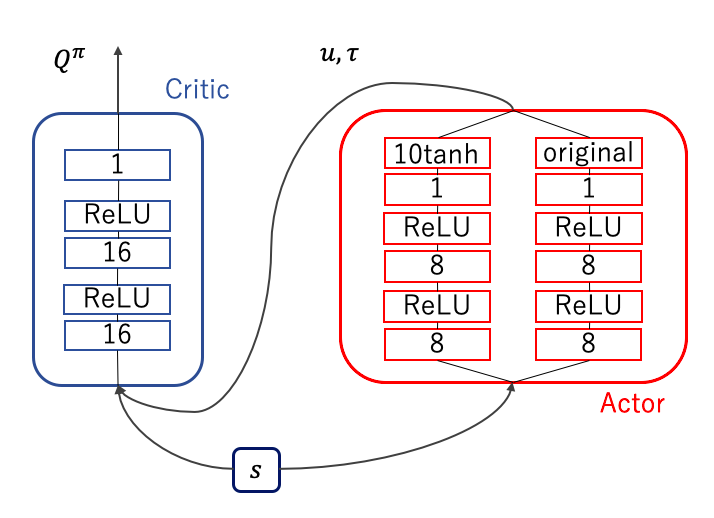
\includegraphics[width=10cm]{model.png}
 	\caption{Agent Model} \label{NN}
\end{figure}\\
The activation function "original" shown in Fig \ref{NN} is defined as $0.99 \times \textrm{sigmoid} + 0.01$ to meet upper and lower limits of interval.


\section{Consideration}
% 小さいノイズの結果であることを明示する
In this section, we study the effectiveness of the reinforcement learning approach to the optimal self-triggered control problem. We conduct numerical experiments and review the results for the cases of linear and nonlinear control systems, respectively. In both cases, the communication interval is allowed to be $0.01 (s) \sim 1.0 (s)$. 

\subsection{Linear Case}
First, we adopt reinforcement learning to self-triggered control for linear system. The control object is
\begin{equation}
	\dot{s} = As + Bu = \begin{bmatrix}-1& 4 \\ 2 & -3\end{bmatrix}s + \begin{bmatrix}2 \\ 4\end{bmatrix}u.
\end{equation}
Here, the input signal $u$ is limited to $-10 \sim 10$.

\subsubsection{Initial Policy}
For learning efficiency, we use $\pi_{\textrm{init}}$ such that
\begin{equation}
	\pi_{\textrm{init}} = \begin{bmatrix}-Ks&0.01\end{bmatrix}
\end{equation}
where $K$ is a feedback gain calculated by Linear Quadratic Regulator. This policy stabilize the system (really??).

\subsubsection{Learned Policy}

\subsubsection{Comparison with Naiive Model Based Control}






\subsection{Non-Linear Case}
In this subsection, we investigate whether the self-triggered control law can be learned by reinforcement learning even when the control target is extended to non-linear systems, especially control affine systems. We consider an inverted pendulum, whose state-space representation is
\begin{equation}
	\odif{}{t}\begin{pmatrix}\theta \\ \dot{\theta}\end{pmatrix} = 
		\begin{pmatrix}\dot{\theta} \\ \frac{3g}{2l}\sin{\theta} + \frac{3}{ml^2}a \end{pmatrix} \label{pendulum}.
\end{equation}
Therefore, for an inverted pendulum, the state variable $s$ is considered to be $\begin{pmatrix}\theta & \dot{\theta}\end{pmatrix}^{\top}$.
\par
As in the linear case, the input signal $u$ is limited to $-10 \sim 10$.

\subsubsection{Initial Policy}
For learning efficiency, we use $\pi_{\textrm{init}}$ such that
\begin{equation}
	\pi_{\textrm{init}} = \begin{bmatrix}-Ks&0.2\end{bmatrix}
\end{equation}
where $K$ is a feedback gain calculated by Linear Quadratic Regulator. This policy stabilize the system.

\subsubsection{Learned Policy}
Fig \ref{path_1} shows a control path with learned policy, stating from $s_0 = [3., 3.]$.
\begin{figure}[h]
	\centering
 	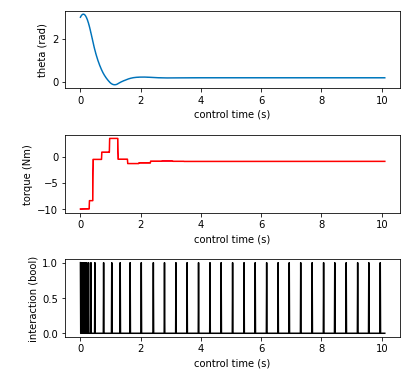
\includegraphics[width=8cm]{path_1.png}
 	\caption{A control path with learned policy $\pi_{\textrm{RL}}$} \label{path_1}
\end{figure}\\
Figure \ref{path_1} shows, from top to bottom, the angle of the pendulum $\theta$, the control input $u$, and the boolean representing interaction. From this figure, we can see that the communication interval is determined flexibly at each interaction.\par
Now, we confirm whether the learned policy $\pi_{\textrm{RL}}$ enlarge the evaluation function $J(\pi)$ compared from the initital policy $\pi_{\textrm{init}}$. Since $J(\pi) = \expect_{s_0}[V^{\pi}(s_0)]$, we generate 500 initial states $s_0$ according to the initial state distribution $d_0$, and average the results of $V^{\pi}(s_0)$. We conduct this approximation of expectation 1000 times. From the result
\begin{equation}
	J(\pi_{\textrm{init}}) = 4.23 \pm 0.083,~J(\pi_{\textrm{RL}}) = 37.12 \pm 0.071 \label{compare_policy}, 
\end{equation}
we can confirm $J(\pi_{\textrm{init}}) < J(\pi_{\textrm{RL}})$. It can be concluded that the policy has been improved.

\subsection{Optimality}
Is the policy $\pi_{\textrm{RL}}$ described in the previous section an optimal? If it is an optimal solution, the policy gradient must be $\bm{0}$. Therefore from equation \eqref{true_pg}, a condition
\begin{equation}
	\nabla_a Q^{\pi_{\textrm{RL}}}(s,a)|_{a=\pi_{\textrm{RL}}(s)} = \bm{0}
\end{equation}
should be met. \par
In order to check whether the policy $\pi_{\textrm{RL}}$ satisfies the condition \eqref{optimality}, we want to know $Q^{\pi_{\textrm{RL}}}(s,a)$. Then, we obtain the approximation of value function $V^{\pi_{\textrm{RL}}}(s) = \sum_{i=0}^{N}\gamma^i r(s_i,\pi_{\textrm{RL}}(s_i))$ with $N$ step simulation:
\begin{equation}
	V^{\pi_{\textrm{RL}}}_{\textrm{ap}}(s) = \sum_{i=0}^{N}\gamma^i r(s_i,\pi_{\textrm{RL}}(s_i)).
\end{equation}
Next, the approximation of $Q^{\pi_{\textrm{RL}}}$ is calculated with $V^{\pi_{\textrm{RL}}}_{\textrm{ap}}$ as following:
\begin{equation}
	Q^{\pi_{\textrm{RL}}}_{\textrm{apd}}(s,a) = r(s,a) + \gamma V^{\pi_{\textrm{RL}}}_{\textrm{ap}}.(s^{\prime})
\end{equation}
Since $\gamma < 1$, $Q^{\pi_{\textrm{RL}}}_{\textrm{apd}}(s,a)$ is a good approximation if the number of simulation steps $N$ is sufficiently large. However, to compute the policy gradient, we need to compute $\nabla_{a}Q^{\pi_{\textrm{RL}}}(s, a)$, while $Q^{\pi_{\textrm{RL}}}_{\textrm{apd}}$ can only be computed the value at $(s,a)$. Then, we approximate the function $Q^{\pi_{\textrm{RL}}}_{\textrm{apd}}(s,a)$ by supervised learning with $Q^{\pi_{\{textrm{RL}}}_{\textrm{apd}}(s,a)$ as the teacher data. This function is defined as $Q^{\pi_{\textrm{RL}}}_{\textrm{ap}}$.\par
Now, when we calculate the policy gradient using $Q^{\pi_{\textrm{RL}}}_{\textrm{ap}}$, we obtain
\begin{equation}
	\expect_{s\sim\rho^{\pi_{\textrm{RL}}}}[
	\nabla_{\theta}\pi_{\textrm{RL}}(s)\nabla_{a}Q^{\pi_{\textrm{RL}}}(s, a)|_{a=\pi_{\textrm{RL}}(s)}] \neq \bm{0}, 
\end{equation}
which means that the policy $\pi_{\textrm{RL}}$ is not an optimal measure. We will discuss the reason for this.

\subsection{Approximation Accuracy of Critic}
Since policy $\pi_{\textrm{RL}}$ makes
\begin{equation}
	\expect_{s\sim\rho^{\pi_{\textrm{RL}}}}[
	\nabla_{\theta}\pi_{\textrm{RL}}(s)\nabla_{a}Q(s,a|\omega)|_{a=\pi_{\textrm{RL}}(s)}] \simeq \bm{0}
\end{equation}
for critic network $Q(s,a|\omega)$, it is a optimal solution to make the approximated gradient be 0. Therefore, the reason why we could not learn the optimal strategy is considered to be the low approximation accuracy of critic. In this experiment, the exploration noise is given as $\sim$, and its scale is small. This leads to a bias in the distribution of the action $a$ in the replay buffer. For example, the distribution of actions experienced in the neighborhood of $s=\begin{bmatrix}0 & 0\end{bmatrix}$ is shown in Figure \ref{data_distribution}.
\begin{figure}[h]
	\centering
 	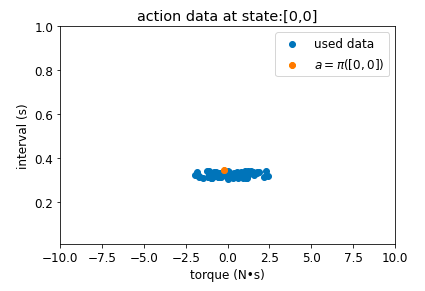
\includegraphics[width=8cm]{data_distribution.png}
 	\caption{Action distribution in replay buffer around $s=[0~0]$.} \label{data_distribution}
\end{figure}\\
Since the approximation accuracy of 
\begin{equation}
	\nabla_{a} Q(s,a|\omega)|_{a=\pi_{\theta}(s)}
\end{equation}
is crucial for the calculation of the policy gradient, the problem is the lack of data around $a=\pi_{\theta}(s)$ which is represented by the orange dot in Figure \ref{data_distribution}.


\subsection{Ingenuity}
We see that small scale exploration noise leads low accuracy of critic's approximation. However, as we confirmed in section \ref{sec:exploration}, large scale exploration noise cause problem of experience distribution. Here, by using the information of the control target, we consider to devise a exploration method. \par
The ideal distribution of replay buffer meets following 2 conditions:
\begin{enumerate} 
	\item The distribution of state $s$ is similar to discounted distribution $\rho^{\pi}(s)$
	\item The variance of action $a$ is large for each state $s$.
\end{enumerate}
Therefore, we propose a method to control the noise scale inversely proportional to the gradient of the state $s^{\prime}$ of the next step with respect to the change of input $a$. 
\begin{equation}
	e \sim \frac{1}{c\|g\|+1} \mathcal{N}(0,1)
\end{equation}
where $g = \frac{ds^{\prime}}{da}$, $c$ is a hyper parameter. \par
As a result of reinforcement learning using this search method, the obtained policy $\pi_{\textrm{MBRL}}$ achieve
\begin{equation}
	J(\pi_{\textrm{MBRL}}) = 68.10 \pm 0.018 \label{ingenuity}.
\end{equation}


\section{Conclusion}
本稿では, 最適セルフトリガー制御に対する強化学習



%%% Acknowledgments %%%%%%%%%%%%%%%%%%%%%%%%%%%%%%%%%%%%%%%%%%%%%%%%%%%%%%%%%%%%%
\acknowledgment
The author would like to express his sincere gratitude to Professor
Yoshito Ohta and Assistant Professor Kenji Kashima for their helpful advices.

%%% References %%%%%%%%%%%%%%%%%%%%%%%%%%%%%%%%%%%%%%%%%%%%%%%%%%%%%%%%%%%%%%%%%%
\addcontentsline{toc}{section}{\refname} % Add to the table of contents.
                                         % Delete if you use chapter option.
\begin{thebibliography}{10}
\bibitem{Q}
C. J. Watkins, and P. Dayan. Q-learning. \textit{Machine Learning}, vol. 8, no. 3-4, pp. 279-292, 1992.
\bibitem{DQN}
V. Minh, K. Kavukcouglu, D. Silver. et al.. “Human-level control through deep reinforcement learning." \textit{Nature 518}, pp.529-533, 2015.
\bibitem{DPG}
D. Silver, G. Lever, N. Heess, T. Degris, D. Wierstra, et al.. “Deterministic Policy Gradient Algorithms." \textit{ICML Beijing, China.}, 2014, Beijing.
\bibitem{DDPG}
T. P. Lillicrap, J. J. Hunt, A. Pritzel, N.Heess, T. Erez, Y. Tassa, D. Silver, and D. Wierstra. Continuous control with deep reinforcement learning. \textit{International Conference on Learning Representations}, 2015.
\bibitem{off-PAC}
T. Degris, M. White and R. Sutton. “Off-Policy Actor-Critic." \textit{ICML Edinburgh, United Kingdom}, 2012.
\bibitem{approximation}
R. S. Sutton, D. McAllester, S. Singh, and Y. Mansour. "Policy gradient methods for reinforcement learning with function approximation." \textit{In Advances in Neural Information Processing Systems}, 2000.
\bibitem{Adam}
D. P. Kingma and J. Ba. “Adam: A Method for Stochastic Optimization." \textit{arXiv preprint arXiv: 1412.6980}, 2014.

\end{thebibliography}
%%% If you want to use BibTeX, delete the above and insert code here.
%% \bibliographystyle{...}
%% \bibliography{...}

%%% Appendix %%%%%%%%%%%%%%%%%%%%%%%%%%%%%%%%%%%%%%%%%%%%%%%%%%%%%%%%%%%%%%%%%%%%
%%% If you don't need appendices, delete the below.
\appendix

\section{Appendix}
This is an appendix. This is a citation~\cite{polya1945}.

\begin{table}[htbp]
  \caption{This is a table.}
  \centering
  \begin{tabular}{c|cc}
      &  A  &  B \\
    \hline
    C &  70 & 80 \\
    D & 100 &  0
  \end{tabular}
\end{table}

%%% End of body %%%%%%%%%%%%%%%%%%%%%%%%%%%%%%%%%%%%%%%%%%%%%%%%%%%%%%%%%%%%%%%%%
\fi
\ifoutputcover
\cleardoublepage
%%% Covers and abstract for submission %%%%%%%%%%%%%%%%%%%%%%%%%%%%%%%%%%%%%%%%%%
\makecover                      % Cover
\makespine[\numberofspines]     % Spine
\fi
\ifoutputabstractforsubmission
\makeabstractforsubmission      % Abstract for submission
\fi
\end{document}
